\chapter{Sprint 6 : Réorganiser/simplifier le pipeline de PROD/PREPROD}
\section{Introduction}
Dans le cadre du dernier sprint, l'équipe s'est concentrée sur une revue complète de la stratégie de déploiement pour le projet SCRIBE. L'objectif principal était de faciliter et d'améliorer le processus de déploiement en environnement de production (PROD), tout en offrant aux développeurs la possibilité de stocker et de déployer facilement des versions de livrables buildées sur les environnements de développement, de test et de production. Ce chapitre explore en détail les objectifs, le backlog, les étapes de réalisation et les résultats obtenus au cours de ce sprint
\section{Analyse des besoins}
Dans cette section, nous allons aborder les objectifs et le backlog de ce sprint.
\subsection{Objectif de sprint 6}
L'objectif majeur de ce sprint était de repenser et d'améliorer la stratégie de déploiement pour le projet SCRIBE. Cela impliquait de faciliter le processus de déploiement en environnement PROD pour l'équipe d'exploitation, tout en offrant aux développeurs un mécanisme pour stocker et déployer des versions de livrables buildées sur différents environnements (DEV, QPM, PREPROD et PROD).

\subsection{Backlog Sprint 6}
\normalsize{Afin de bien organiser le travail durant ce sprint, nous allons établir le Backlog du sprint 6 illustré par le tableau \ref{tab:sprintBacklog6}.
\newpage
\begin{longtable}{|>
{\centering}m{0.085\linewidth}|>
{\centering}m{0.3\linewidth}|>{\centering}m{0.085\linewidth}|>
{\centering}m{0.2\linewidth}|c|}
\hline
ID User Story & User story & ID tâche & Tâche & Priorité \\
\hline
\multirow{3}{*}{6.1} & \multirow{3}{\linewidth}{ {En tant que  membre de l'équipe d'exploitation, je peux lancer le pipeline de déploiement
en PROD pour le projet "Scribe" avec plus de facilité et de lisibilité.}} & 6.1.1 &  Faire les modification nécessaire au niveau gitlab ci. & Haute \\ 
\cline{3-5}
      & & 6.1.2 & Tester l'impact des modifications sur la durée d'exécution. & Moyenne \\
\hline
\multirow{3}{*}{6.2} & \multirow{3}{\linewidth}{ {En tant que  membre de l'équipe d'exploitation, je peux génèrer un livrable unique à tous les
environnements.}} & 6.2.1 &  Configurer le job "release" pour deployer les livrable au niveau Jfrog. & Haute \\ 
\cline{3-5}
      & & 6.2.2 & Tester le job "release". & Moyenne \\

\cline{3-5}
      & & 6.2.3 & Créer une nouvelle branche Git nommée "deploy\_livrable" à partir de la branche principale du projet. & Haute \\
\cline{3-5}
      & & 6.2.4 & Configurer le pipeline du branche "deploy\_livrable" visant à télécharger et déployer les livrables à partir de JFrog vers les environnements cibles. & Haute \\
\cline{3-5}
      & & 6.2.5 & Tester le deploiement pour chaque groupe et environnement cible. . & Moyenne \\
\hline
\caption{Backlog du Sprint 6}
\label{tab:sprintBacklog6}
\end{longtable}
\section{Réalisation}
Pour la première partie, nous avons repensé le processus de déploiement en environnement PROD en simplifiant les scripts et en intégrant une interface utilisateur conviviale pour lancer le pipeline de déploiement. Cette refonte a permis à l'équipe d'exploitation de déployer en PROD de manière plus intuitive et transparente.
\subsection{Alléger le pipeline de PROD}
Un examen minutieux des étapes du pipeline de déploiement en PROD a été effectué pour identifier les étapes qui pouvaient être optimisées ou supprimées. Cela a permis de mettre en évidence les parties du processus qui ajoutaient de la complexité et n'étaient pas essentielles pour le déploiement réussi en PROD.\\
le tableau \ref{tab:les-etapes-a-supprimer} illustre les etape à supprimer
\begin{longtable}{|>{\centering\arraybackslash}m{0.2\linewidth}|>{\centering\arraybackslash}m{0.2\linewidth}|>{\centering\arraybackslash}m{0.2\linewidth}|}
\hline
Unit Test & Test & Deploy \\
\hline
agh\_unit\_test & Sonar & Test Fonctionnels \\
\hline
\caption{Les Étapes à Supprimer}
\label{tab:les-etapes-a-supprimer}
\end{longtable}

La figure \ref{PROD} illustre le processus simplifié de lancement du pipeline de déploiement en environnement de production (PROD).

\begin{figure}[H]
    \centering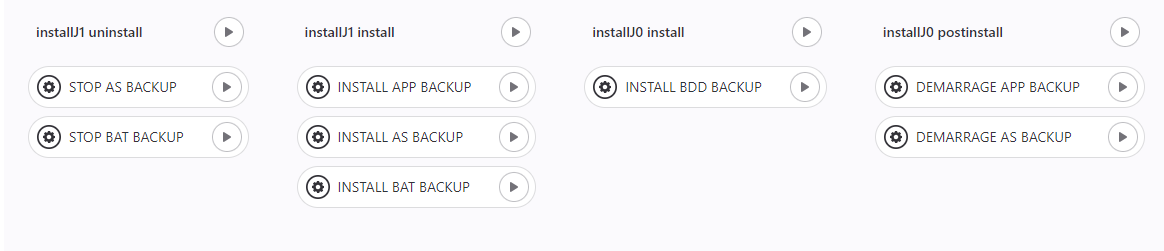
\includegraphics[scale=0.55]{img/PROD.PNG}
    \caption{Pipeline PROD }
    \label{PROD}
 \end{figure}
 \subsection{Un livrable unique à tous les environnements}
 Pour atteindre l'objectif de générer un unique colis/livrable déployé sur tous les environnements (DEV, QPM, PREPROD et PROD) en utilisant une version préalablement buildée stockée dans un référentiel, nous avons mis en place un processus structuré. \\
 Voici les étapes clés de cette réalisation :
 \newpage
 \subsubsection{Ajout du Job "release-repo" :}
 Tout d'abord, dans le cadre du pipeline du projet SCRIBE, nous avons introduit un nouveau job nommé "release-repo". Ce job est essentiel pour la gestion des versions préalablement buildées et stockées dans un référentiel centralisé. La capture ci-dessous illustre le contenu et le fonctionnement de ce job.
La figure \ref{pipeline Scribe} illustre le pipeline SCRIBE montrant le nouveau job "release-repo".
\begin{figure}[H]
    \centering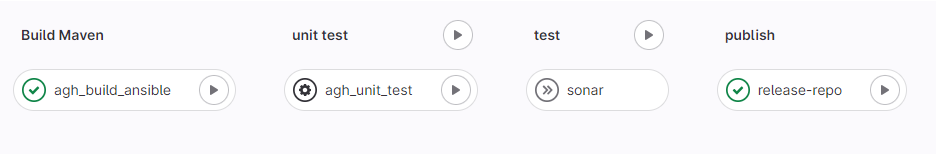
\includegraphics[scale=0.55]{img/pipeline Scribe.PNG}
    \caption{Pipeline Sribe }
    \label{pipeline Scribe}
 \end{figure}
Après l'exécution du job "release-repo", la figure \ref{jar} illustre le déploiement des livrables au format JAR vers JFrog.
\begin{figure}[H]
    \centering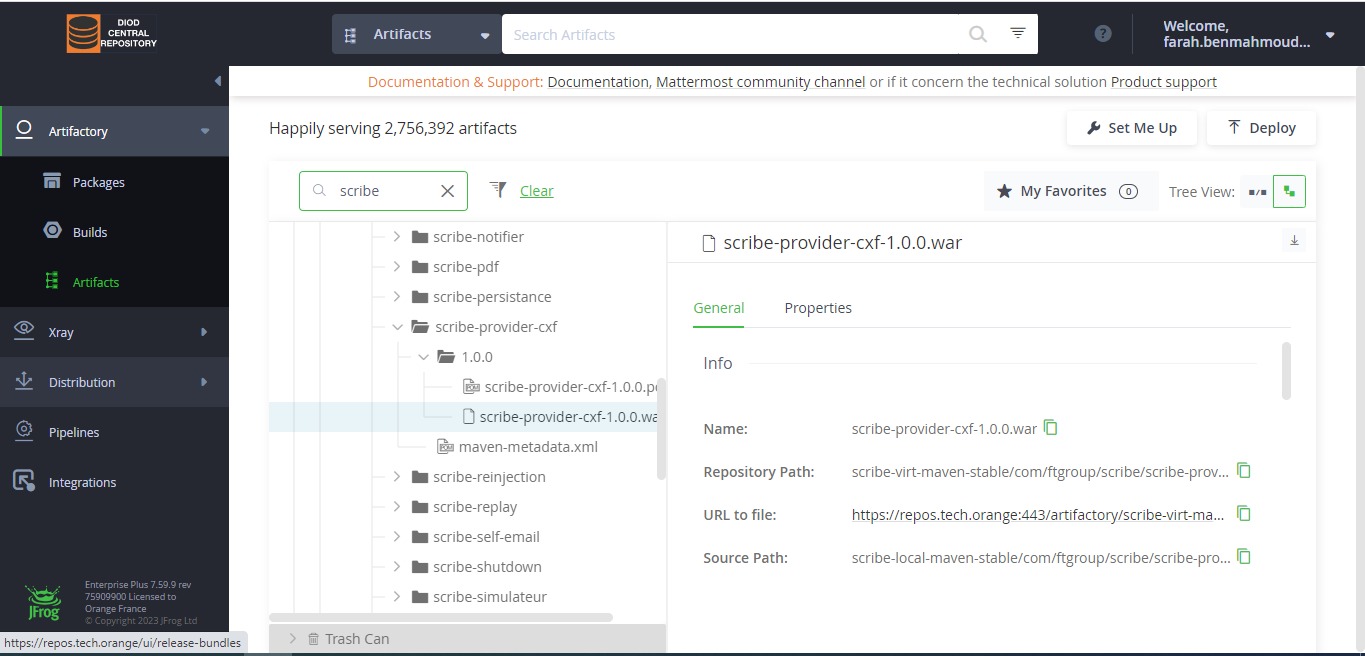
\includegraphics[scale=0.4]{img/frog_jar.PNG}
    \caption{le déploiement des livrables au format JAR vers JFrog}
    \label{jar}
 \end{figure}
 \newpage
Ainsi que le déploiement des livrables au format WAR vers JFrog comme montre la figure \ref{warr}

 \begin{figure}[H]
    \centering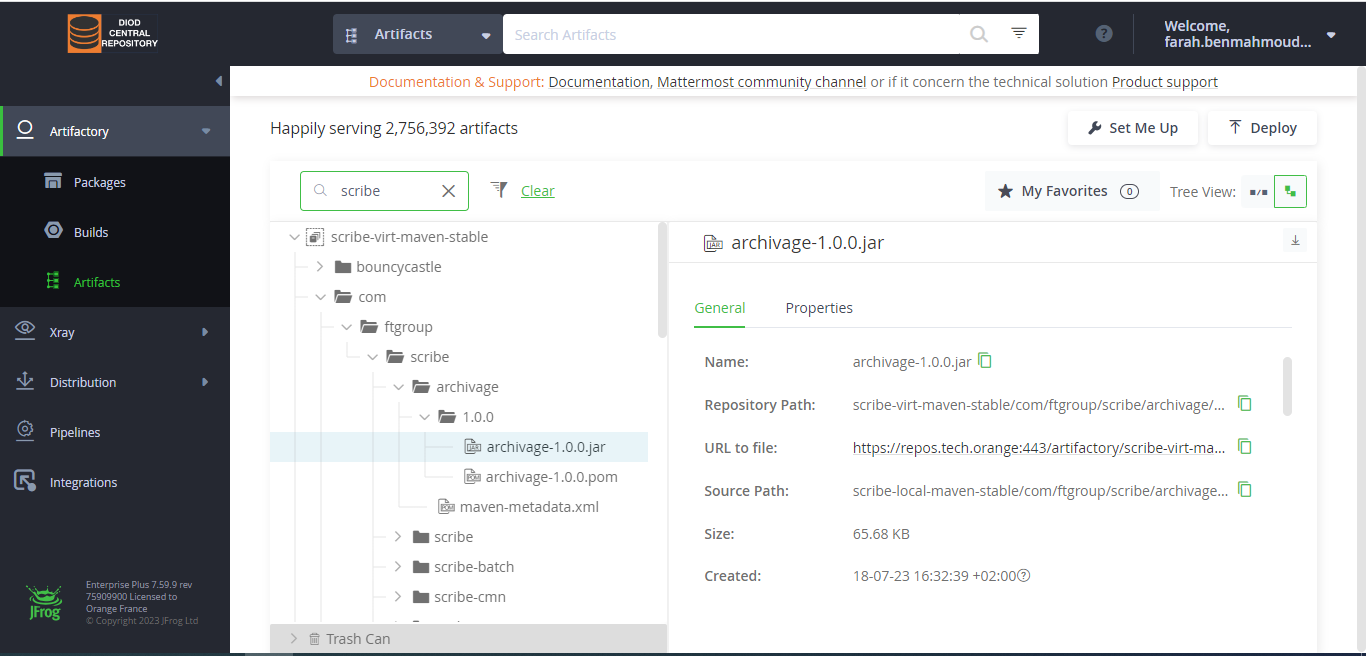
\includegraphics[scale=0.4]{img/jfrog_war.PNG}
    \caption{le déploiement des livrables au format WAR vers JFrog}
    \label{warr}
 \end{figure}
\subsubsection{Déploiement des Livrables dans JFrog Artifactory :}
Pour faciliter le déploiement des livrables sur tous les environnements, nous avons créé une branche distincte nommée "deploy\_livrable". Cette branche est conçue pour télécharger et déployer les livrables quel que soit le projet et l'environnement appropriés.
\subsubsection{Déploiement selon l'Environnement :}
\begin{itemize}
    \item \textbf{Environnement PROD :} Un pipeline spécifique a été configuré dans la branche "deploy\_livrable" pour le déploiement en environnement de production (PROD). Cette configuration assure que les versions préalablement buildées sont récupérées depuis le référentiel JFrog Artifactory et déployées étape par étape sur le serveur PROD. \\
    La figure \ref{Pipeline SCRIBE dans la branche "deploy_livrable" en Environnement PROD} illustre le pipeline SCRIBE au niveau de la branche "deploy\_livrable" en environnement PROD
\begin{figure}[H]
    \centering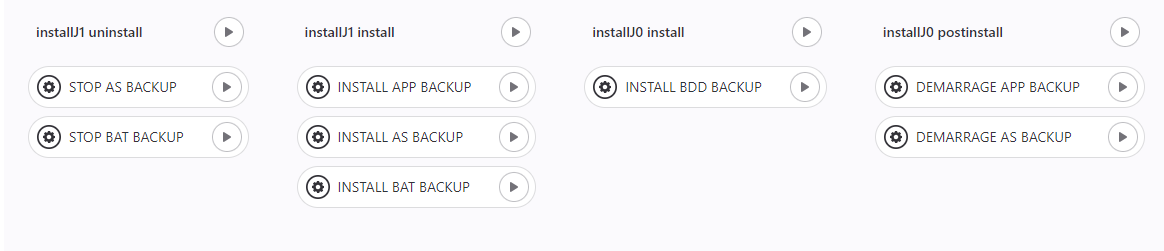
\includegraphics[scale=0.55]{img/PROD.PNG}
    \caption{Pipeline SCRIBE dans la branche "deploy\_livrable" en Environnement PROD}
    \label{Pipeline SCRIBE dans la branche "deploy_livrable" en Environnement PROD}
 \end{figure}
 \newpage
 \item \textbf{Environnement QPM et PREPROD :} Pour les environnements de qualité et de pré-production (QPM et PREPROD), un processus de déploiement séquentiel a été mis en place. Les livrables sont téléchargés depuis le référentiel JFrog Artifactory et déployés en plusieurs étapes pour garantir la stabilité et la cohérence. \\
    La figure \ref{Pipeline SCRIBE dans la branche "deploy_livrable" en Environnement PREPROD et QPM} illustre le pipeline SCRIBE au niveau de la branche "deploy\_livrable" en environnement PRE PROD et QPM
\begin{figure}[H]
    \centering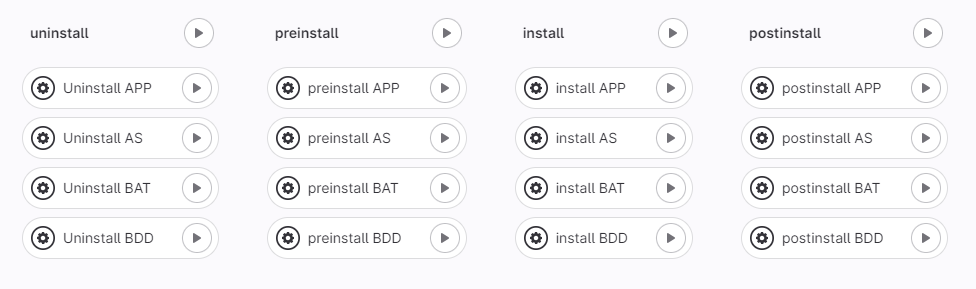
\includegraphics[scale=0.55]{img/PRE QPM.PNG}
    \caption{Pipeline SCRIBE dans la branche "deploy\_livrable" en Environnement PRE PROD et QPM}
    \label{Pipeline SCRIBE dans la branche "deploy_livrable" en Environnement PREPROD et QPM}
 \end{figure}
 \item \textbf{Environnements DEV, DEV1 et DEV2 :} Enfin, pour les environnements de développement (DEV, DEV1 et DEV2), le déploiement des fichiers JAR et WAR est géré au niveau du serveur, conformément aux besoins spécifiques de ces environnements.\\
    La figure \ref{Pipeline SCRIBE dans la branche "deploy_livrable" en Environnement DEV, DEV1 et DEV2} illustre le pipeline SCRIBE au niveau de la branche "deploy\_livrable" en environnement DEV, DEV1 et DEV2
\begin{figure}[H]
    \centering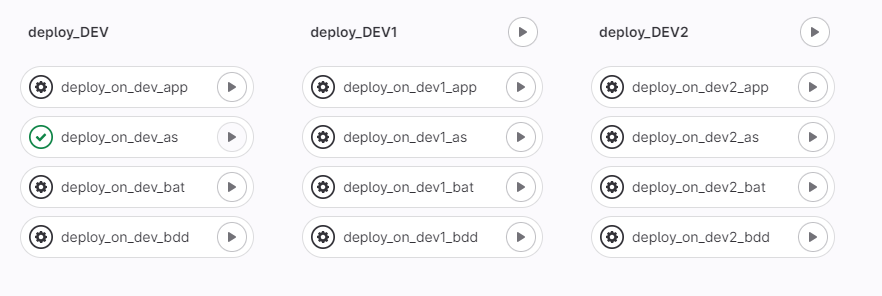
\includegraphics[scale=0.55]{img/deploy livable.PNG}
    \caption{Pipeline SCRIBE dans la branche "deploy\_livrable" en Environnement DEV, DEV1 et DEV2}
    \label{Pipeline SCRIBE dans la branche "deploy_livrable" en Environnement DEV, DEV1 et DEV2}
 \end{figure}
    La figure \ref{Le déploiement des fichiers JAR au niveau de l'environnement DEV.} illustre le du déploiement des fichiers JAR au niveau de l'environnement DEV.
\begin{figure}[H]
    \centering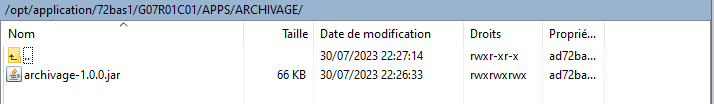
\includegraphics[scale=0.55]{img/deploy Archivage.PNG}
    \caption{Le déploiement des fichiers JAR au niveau de l'environnement DEV.}
    \label{Le déploiement des fichiers JAR au niveau de l'environnement DEV.}
 \end{figure}
    La figure \ref{Le déploiement des fichiers WAR au niveau de l'environnement DEV.} illustre le du déploiement des fichiers WAR au niveau de l'environnement DEV.
\begin{figure}[H]
    \centering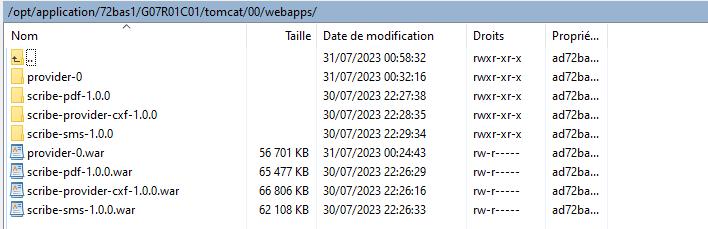
\includegraphics[scale=0.55]{img/war.PNG}
    \caption{Le déploiement des fichiers WAR au niveau de l'environnement DEV.}
    \label{Le déploiement des fichiers WAR au niveau de l'environnement DEV.}
 \end{figure}

Cette réalisation a considérablement simplifié le processus de déploiement, assurant l'utilisation des mêmes versions préalablement buildées sur tous les environnements. Cette uniformité contribue à minimiser les erreurs, à garantir la cohérence et à améliorer l'efficacité globale du déploiement du projet SCRIBE.
\end{itemize}

\section{Conclusion}
Au cours de ce sprint, nous avons réorganisé et simplifié le pipeline de production/préproduction en réduisant la complexité du pipeline de production, résultant en la génération d'un seul package/livrable déployé de manière cohérente sur nos quatre environnements : DEV, QPM, PREPROD et PROD.